\section{守恒律问题}
\label{sec:cons-problem}

一段路上的车辆数只会因为有车从两端进出而改变。把这句话写成数学，就得到本章的方程。

\paragraph{从区间收支到方程}
设$u(x,t)$是$t$时刻$x$处的密度，例如单位长度上的车辆数。单位时间内向右穿过$x$点的量称为\term{通量}（flux）。本章假设通量只通过密度依赖位置和时间，写成$F(u(x,t))$，其中$F:\mathbb{R}\to\mathbb{R}$是给定的函数。

任取区间$[a,b]$，如图~\ref{fig:cons-balance}。区间内的总量只因两端的进出而变化，左端流入，右端流出：
\begin{equation}
  \frac{\mathrm{d}}{\mathrm{d}t}\int_a^b u(x,t)\,\mathrm{d}x=F(u(a,t))-F(u(b,t)).
  \label{eq:cons-balance}
\end{equation}

\begin{BookInlineFigure}
  \centering
  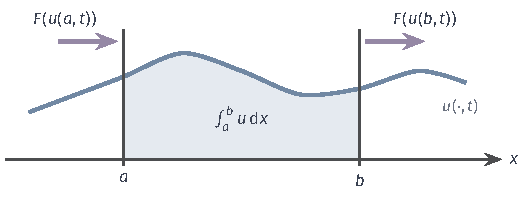
\includegraphics[width=89.8mm]{figures/06-differential-equations/02-partial-differential-equations/tikz/cons-balance/figure.pdf}
  \caption{区间上的收支。蓝线是某一时刻的密度$u(\cdot,t)$，浅蓝区域的面积是区间$[a,b]$内的总量。紫色箭头表示穿过两个端点的通量，左端流入增加总量，右端流出减少总量。}
  \label{fig:cons-balance}
\end{BookInlineFigure}

式~\eqref{eq:cons-balance}没有对$x$求导，也不要求$u$连续，只要积分和端点值有意义就能写出来。后面处理间断时正要回到这一点。现在先假设$u$和$F$都是$C^1$的，把右端写成$\partial_xF(u)$的积分：
\[
  \int_a^b\bigl(\partial_tu+\partial_xF(u)\bigr)\,\mathrm{d}x=0 .
\]

区间$[a,b]$是任取的，被积函数又连续。如果被积函数在某一点不为零，在该点附近的小区间上积分就不为零，与上式矛盾。于是得到
\begin{equation}
  \partial_tu+\partial_xF(u)=0,\qquad x\in\mathbb{R},\ t>0.
  \label{eq:cons-law}
\end{equation}

再给定初始分布
\begin{equation}
  u(x,0)=u_0(x),\qquad x\in\mathbb{R},
  \label{eq:cons-initial}
\end{equation}
式~\eqref{eq:cons-law}与~\eqref{eq:cons-initial}合起来就是\term{标量守恒律}（scalar conservation law）的初值问题。“守恒”一词来自式~\eqref{eq:cons-balance}：若$u$在无穷远处衰减，使两端的通量趋于同一个值，令$a\to-\infty$、$b\to\infty$，则右端为零，全直线上的总量$\int_{\mathbb{R}}u\,\mathrm{d}x$不随时间变化。

\paragraph{通量决定传播速度}
$C^1$解可以用链式法则展开$\partial_xF(u)$，得到
\begin{equation}
  \partial_tu+F'(u)\,\partial_xu=0.
  \label{eq:cons-quasilinear}
\end{equation}

把它与第~\ref{chap:transport-equations}章的输运方程$\partial_tu+v\,\partial_xu=0$对照，形式完全相同，只是速度$v$换成了$F'(u)$。$F'(u)$是密度$u$上的小扰动的传播速度。差别在于，输运方程的$v$事先已知，这里的速度要等解出$u$之后才知道。下面三种通量显示了通量形状带来的不同，见图~\ref{fig:cons-fluxes}。

\begin{itemize}
  \item 线性通量$F(u)=cu$：速度$F'(u)=c$是常数，方程退回到恒定速度的输运方程。
  \item \term{Burgers方程}（Burgers equation）的通量$F(u)=u^2/2$：速度$F'(u)=u$，场值本身就是传播速度。可以把$u$想成一维粒子各自的速度，每个粒子不受力，匀速前进。
  \item 车流通量$F(u)=u(1-u)$，其中$u\in[0,1]$是归一化密度：车速为$1-u$，空路上最快，堵死时为零，流量等于密度乘车速。
\end{itemize}

\begin{BookInlineFigure}
  \centering
  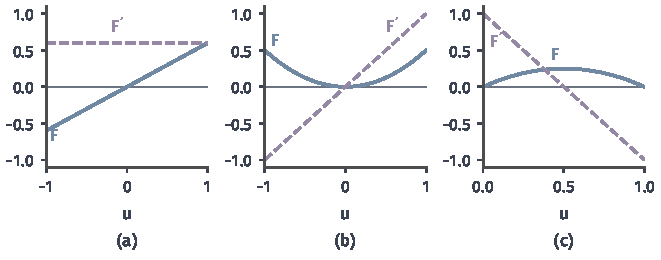
\includegraphics[width=112mm]{figures/06-differential-equations/02-partial-differential-equations/matplotlib/cons-fluxes/figure.pdf}
  \caption{三种通量及其传播速度。蓝色实线是通量$F$，紫色虚线是传播速度$F'$。(a)线性通量$F=0.6u$，速度为常数。(b)Burgers通量$F=u^2/2$，速度等于$u$，$F$是凸函数。(c)车流通量$F=u(1-u)$，速度$1-2u$随密度减小，$F$是凹函数。}
  \label{fig:cons-fluxes}
\end{BookInlineFigure}

车流的例子说明，扰动的传播速度和粒子的速度是两回事。取$u=3/4$，每辆车以速度$1-u=1/4$向前开，而密度扰动的传播速度是
\[
  F'(3/4)=1-2\cdot\frac34=-\frac12 ,
\]
它是负的。车在向前走，密度的变化却向后传，这就是堵车的尾部向后蔓延的原因。Burgers方程里两者恰好相同，读图和手算都最简单，所以本章用
\begin{equation}
  \partial_tu+\partial_x\Bigl(\frac{u^2}{2}\Bigr)=0
  \label{eq:cons-burgers}
\end{equation}
作贯穿全章的例子。

\paragraph{讨论的范围}
本章只讨论一维标量方程。未知量是向量的守恒律系统有多族速度不同的波，它们彼此耦合，本章后面的唯一性论证没有对应物。多维标量方程的熵解理论仍然成立，但间断不再是一条曲线，左右两侧的次序也不复存在，一维的显式构造不能照搬。下文的条件和结论都只针对一维标量问题。
